\documentclass[12pt]{article}
\usepackage{times} 			% use Times New Roman font

\usepackage[margin=1in]{geometry}   % sets 1 inch margins on all sides
\usepackage{hyperref}               % for URL formatting
\usepackage[pdftex]{graphicx}       % So includegraphics will work
\setlength{\parskip}{1em}           % skip 1em between paragraphs
\usepackage{indentfirst}            % indent the first line of each paragraph
\usepackage{datetime}
\usepackage[small, bf]{caption}
\usepackage{listings}               % for code listings
\usepackage{xcolor}                 % for styling code
\usepackage{multirow}
\usepackage{float}
\usepackage{longtable}
%New colors defined below
\definecolor{backcolour}{RGB}{246, 246, 246}   % 0xF6, 0xF6, 0xF6
\definecolor{codegreen}{RGB}{16, 124, 2}       % 0x10, 0x7C, 0x02
\definecolor{codepurple}{RGB}{170, 0, 217}     % 0xAA, 0x00, 0xD9
\definecolor{codered}{RGB}{154, 0, 18}         % 0x9A, 0x00, 0x12

%Code listing style named "gcolabstyle" - matches Google Colab
\lstdefinestyle{gcolabstyle}{
  basicstyle=\ttfamily\small,
  backgroundcolor=\color{backcolour},   
  commentstyle=\itshape\color{codegreen},
  keywordstyle=\color{codepurple},
  stringstyle=\color{codered},
  numberstyle=\ttfamily\footnotesize\color{darkgray}, 
  breakatwhitespace=false,         
  breaklines=true,                 
  captionpos=b,                    
  keepspaces=true,                 
  numbers=left,                    
  numbersep=5pt,                  
  showspaces=false,                
  showstringspaces=false,
  showtabs=false,                  
  tabsize=2
}

\lstset{style=gcolabstyle}      %set gcolabstyle code listing

% to make long URIs break nicely
\makeatletter
\g@addto@macro{\UrlBreaks}{\UrlOrds}
\makeatother

% for fancy page headings
\usepackage{fancyhdr}
\setlength{\headheight}{13.6pt} % to remove fancyhdr warning
\pagestyle{fancy}
\fancyhf{}
\rhead{\small \thepage}
\lhead{\small HW8, Adeniran Adeniyi}  % EDIT THIS, REPLACE # with HW number
\chead{\small CS 532, Spring 2021} 

%-------------------------------------------------------------------------
\begin{document}

\begin{centering}
{\large\textbf{HW8 - Clustering}}\\ % EDIT THIS
                                % REPLACE # with HW num and ADD title
Adeniran Adeniyi\\                     % EDIT THIS
Sunday, April 18, 2021 by 11:59pm\\                      % EDIT THIS
\end{centering}

%-------------------------------------------------------------------------

% The * after \section just says to not number the sections
%----------------------------Q1111111111111111111111111111111111

\section*{Q1}
\emph{
\\Generate a list of 100 popular accounts on Twitter. The accounts must be verified, have $<$ 10,000 followers, and have $>$ 5000 tweets.
\\ \\ For example:
https://twitter.com/weiglemc - not verified, 457 followers, 2554 tweets - don't include
https://twitter.com/WNBA - verified (blue checkmark), 672,800+ followers, 77,900+ tweets - could include \\See GET users/lookup, Tweepy's API.lookup\_users(), and User object for details on obtaining this information for a set of accounts.\\ \\
You may also generate this information manually by visiting individual account pages
Because we're trying to cluster the accounts based on the text in their tweets, you should choose several sets of accounts that are similar (political, tech, sports, etc.) to see if they'll get clustered together later.
Save the list of accounts (screen\_names), one per line, in a text file named accounts.txt and upload to your GitHub repo.\\ \\
How did you choose to collect the accounts?\\ \\
What topics/categories do the accounts belong to? \\ \\ You don't need to specify a grouping for each account, but what general topics/categories will you expect to be revealed by the clustering?}
\subsection*{\color{blue}{Answer}}

\lstinputlisting[language=Python,caption=tweetparser.py, label=Q1alist:import,firstnumber=1,firstline=1,lastline=59]{tweetparser.py}
\lstinputlisting[language=Python,caption=gatherId.py, label=Q1blist:import,firstnumber=1,firstline=1,lastline=99]{gatherIds.py}

\subsection*{Discussion}
\emph{In gathering users screen names I did took into consideration of the following:}
    \begin{itemize}
        \item I collected the screen names going through 4 major popular twitter accounts 
        \href{https://twitter.com/WIRED}{WIRED}, \href{https://twitter.com/WNBA}{WNBA}, \href{https://twitter.com/POTUS45}{POTUS45}, and \href{https://twitter.com/future_of_music}{future\_of\_music}
        \lstinputlisting[language=Python,caption=A snap shot of gatherIds.py show these accounts doing screen\_name account extraction, label=Q1clist:import,firstnumber=49,firstline=49,lastline=53]{gatherIds.py}
         following list, I extracted accounts the met the requirement of  being verified, have $>$ 10,000 followers, and have $>$ 5000 tweets 
         \item The function confirm\_usermetsrequiremetn() in tweetparser.py on line 8 to 19 check to make sure the accounts fulfilled these requirement
         \lstinputlisting[language=Python,caption=A snap shot of tweetparser.py that check screen\_name account meets requirements, label=Q1clist:import,firstnumber=8,firstline=8,lastline=19]{tweetparser.py} Imports of the file was made on line 8 of gatherIds.py
         \lstinputlisting[language=Python,caption=A snap shot of gatherIds.py that shows the needed imports, label=Q1clist:import,firstnumber=7,firstline=7,lastline=10]{gatherIds.py}
         \item Function per\_account() produce a text files (names based on the arguement supplied ) that gets stored in Q1 folder
         \item I then merge all the produced files from each of the accounts to form the main accounts.txt file.  Seen in line 55 - 85
         \lstinputlisting[language=Python,caption=A snap shot of gatherIds.py shows the merging process of the files generated  by each account, label=Q1clist:import,firstnumber=55,firstline=55,lastline=85]{gatherIds.py}
    \end{itemize}
\section*{Q2}
\emph{Create Account-Term Matrix  }
\subsection*{\color{blue}{Answer}}
\lstinputlisting[language=Python,caption=generatetweetvector.py, label=Q2alist:import,firstnumber=1,firstline=1,lastline=140]{generatetweetvector.py}
\subsection*{Discussion}
\emph{The code drive started from line 47 to line 133}
    \begin{itemize}
        \item Getting the twitter api authentication at line 50, I passeding secrets.json which contained my twitter consumer\_key and consummer\_secret
        \item Read the account files containing the list of scree\_names while removeing any spaces each account name
        \item From lines 61 to 75, uses a major function called getwordcounts(api,screen\_name). In this function the parse(api,screen\_name) is called. The parse function returns users tweets full text that are not retweets nor replies. When that full tweet text is gotten for a particular user, getwords(tweet) function removes unwanted text from the tweets gotten such as URLS and Mentions. It then extracts word that has at least 3 to 15 length size in each sentence in the tweets and converts them to lower cases. \\ \\The result is stored for each words in a dictionary where by if the word repeats itself again the word(which is the  key of the dictionary) increments the values by one. \\ \\ getwordcounts returns the screen name with a dictionary or words with its frequency count as well.
        \item Moving we count the number of accounts each term appear. I noticed that each works and users account are store in a variable outside the for loop, so basically result gotten gets added on each screen\_names.
        \item It appears to keep track of the overall frequency of the word too for every user combined.
        \item I had done some testing to understand the result for one user in lines 78 to 87 
        \lstinputlisting[language=Python,caption=A snapshot for generatetweetvector.py trying to test the output of sumcounts variable listing out the keys values, label=Q2clist:import,firstnumber=78,firstline=78,lastline=87]{generatetweetvector.py}
        \item Removes stop words (this is calculated, not  gotten from a list of unwanted words) basically getting the word count divided  by the total number of account names gotten from the accounts.txt, once is satisfy a particular fraction between 0.1 and 0.5 the word is added to the group of wordlist
        \item For popularlist, From my deduced test above, I was able to sort the item using a lambda function an placed the result in a list of tuples.It goes from highest to lowest. Next I retried just 1000 row items from the tuples(by slicing) and stored it in the dictionary variable popularlist.
        \lstinputlisting[language=Python,caption=A snapshot for generatetweetvector.py Sort tuples Get 1000 rows Save in dictionary variable popularlist, label=Q2dlist:import,firstnumber=105,firstline=105,lastline=109]{generatetweetvector.py}
        \item Finally, results of popularlist variable words are saved in a text file while tweetdata.txt as a header of the popularlist or words and the screen\_name with count of each word on a single row.
        \item The word i viewed in popularlist.txt makes a lot of sense because it is as a form of connection to politics,sports,music or tech
    \end{itemize}

\section*{Q3}
\emph{
\\Create Dendrogram\\ \\Create an ASCII dendrogram and a JPEG dendrogram that uses hierarchical clustering to cluster the most similar accounts (see Module 12, slides 21, 23). Include the JPEG in your report and upload the ASCII file to GitHub (it will be too unwieldy for inclusion in the report).\\ \\How well did the hierarchical clustering do in grouping similar accounts together? Were there any particularly odd groupings?
}
\subsection*{\color{blue}{Answer}}
 \lstinputlisting[language=Python,caption=question3.py for questions 3 4 and 5, label=Q2dlist:import,firstnumber=1,firstline=1,lastline=532]{question3.py}
 \begin{figure}[H]
            \centering
            % trim and clip are used to crop the image, trim=left bottom right top
            % width sets max width, height will be scaled appropriately
            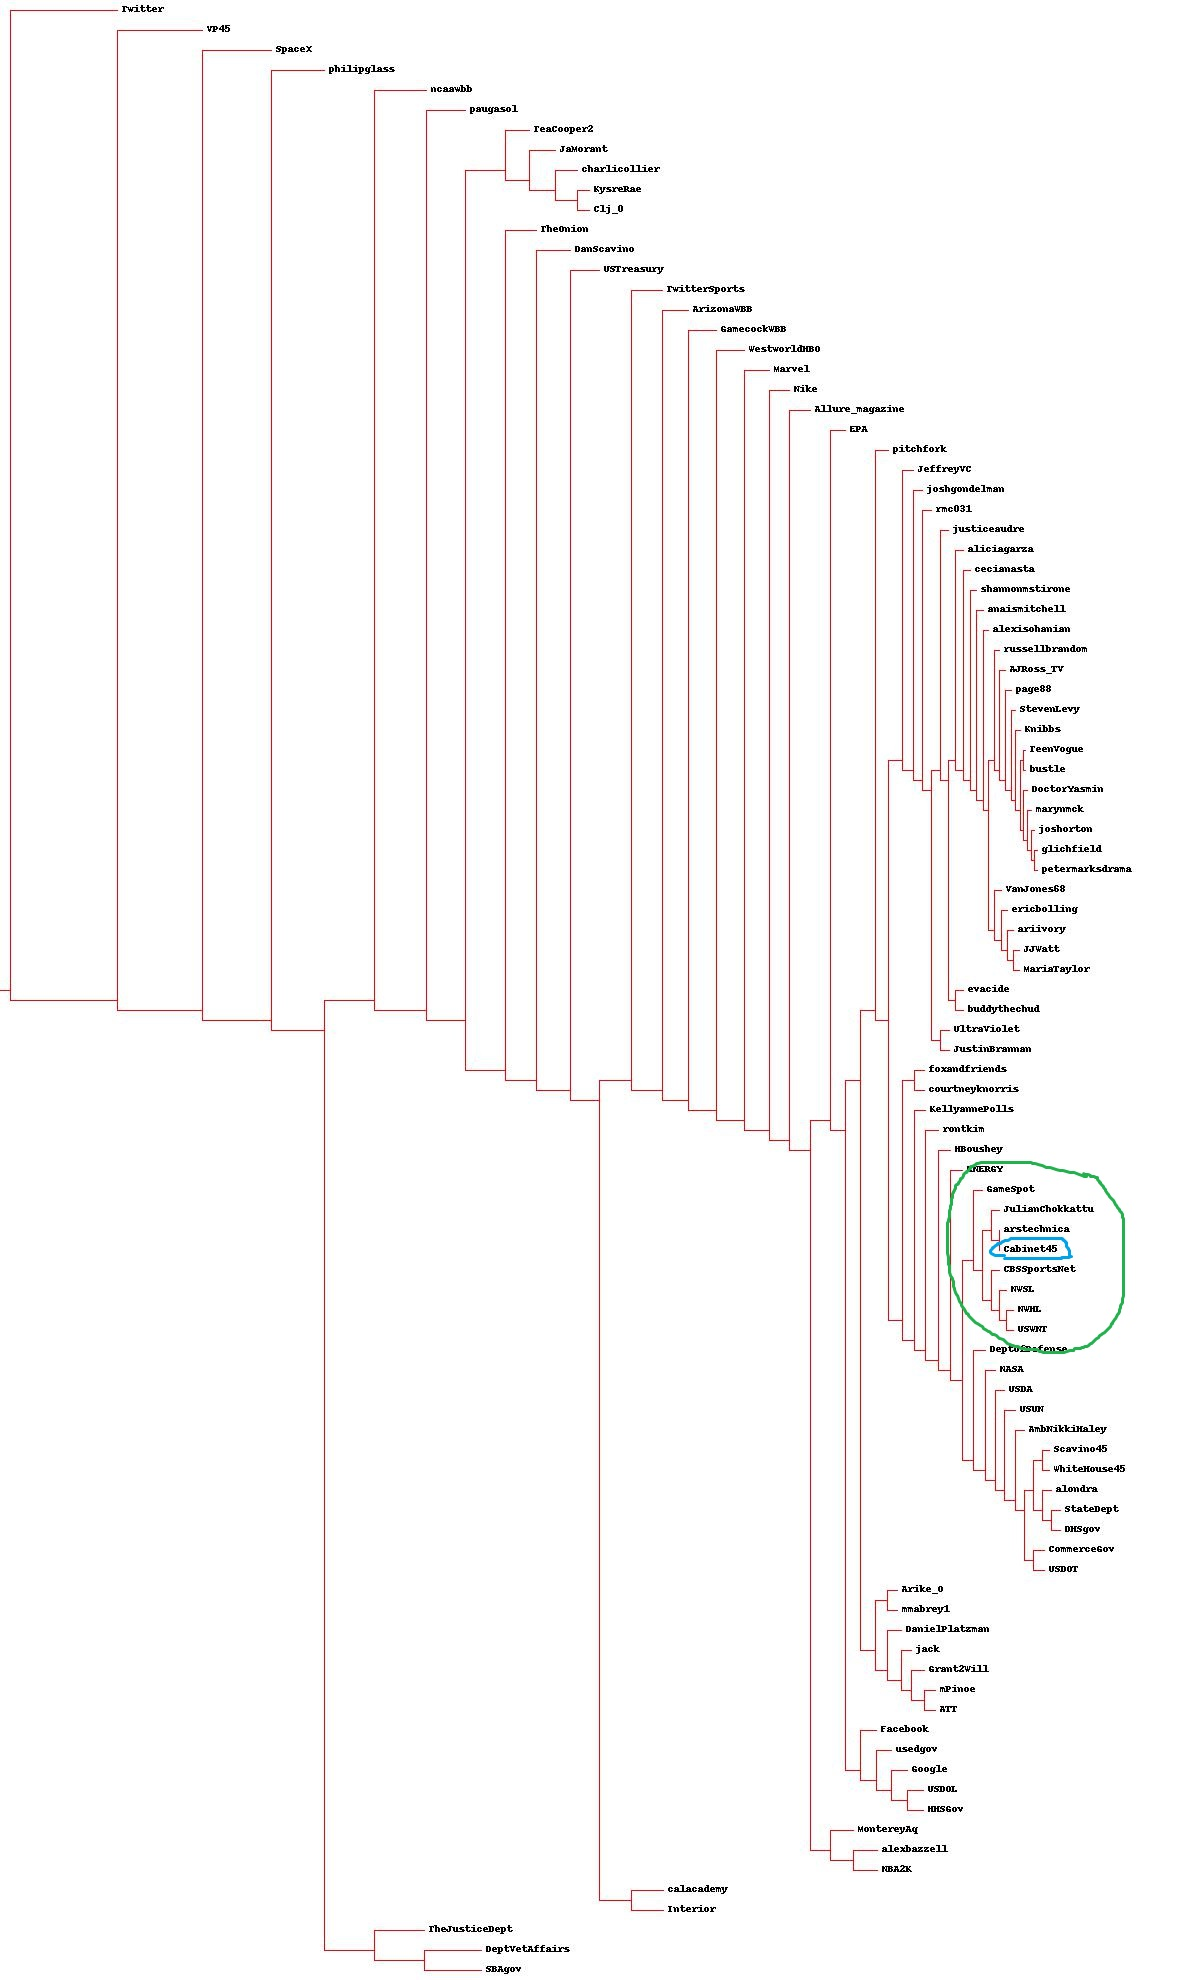
\includegraphics[width=\textwidth,height=\textheight,keepaspectratio]{tweetdataOld.jpeg}
            \caption{ The resulting output for Question 3 twitter account Cabinet45 included}
            \label{fig:1}
\end{figure}
 \begin{figure}[H]
            \centering
            % trim and clip are used to crop the image, trim=left bottom right top
            % width sets max width, height will be scaled appropriately
            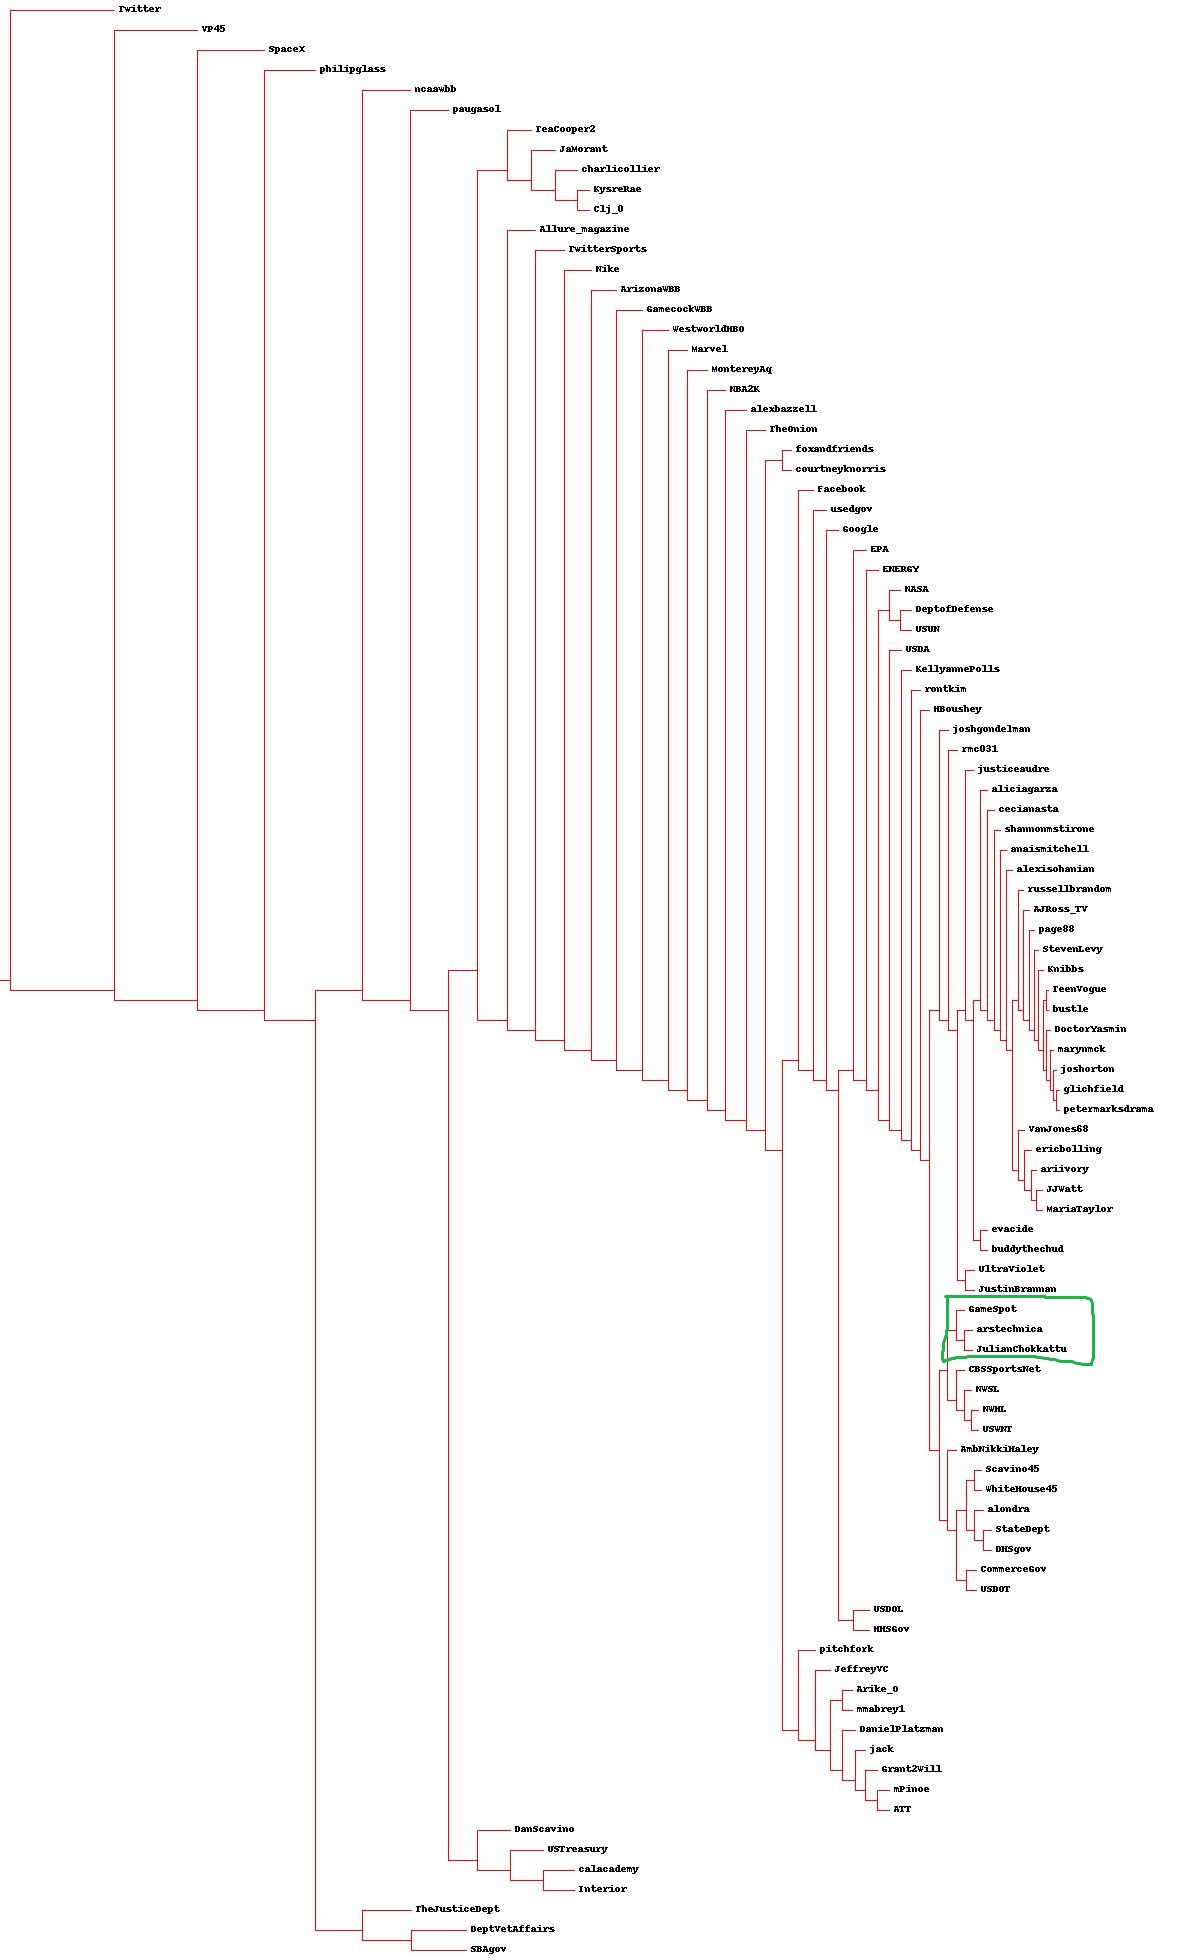
\includegraphics[width=\textwidth,height=\textheight,keepaspectratio]{tweetdata.jpeg}
            \caption{ The resulting output for Question 3 after removing tweet account Cabinet45}
            \label{fig:2}
\end{figure}
\subsection*{Discussion}
\emph{In getting the ASCII and Dendrogram the following had to be put in place:}
    \begin{itemize}
        \item Line 349 to 358 is the drive for the code.
        \lstinputlisting[language=Python,caption= A snapshot question3.py  driver for Q3, label=Q3alist:import,firstnumber=340,firstline=340,lastline=358]{question3.py}
        \item Used the readfile() function to read in the textdata.txt,  it gets all data and returns the usernames as rownames, the words as colnames, and the value as data(data stored as a 2D array of float values).
        \item Next I parsed in data in  hcluster(data) aka hierarchical clustering, this function used the pearson() function when called.
        \\ \\The pearson function takes two vector arrays as arguments and then returns the pearson correlation between these values.\\ \\hcluster() function also uses a bi-cluster class which is an helper for comparing two clusters. \\ \\hcluster does the hierarchical clustering by agglomerative clustering which involves merging the  best  matches cluster with a  new cluster. It repeats this cycle untill there is just one cluster left.
        \item printcluster() function prints recursively the final end product of the hclusters returned function. The printcluster has an argument called labels, the label when removed prints the cluster based on the position number of accounts names but when the label is supplied it prints the actual name of the labels. Print produces the ASCII text of the output. I basically copied and pasted in  a text file.
        \item drawdendrogram() does the similar objective as the printcluster but it produces a jpeg format of the recursive output of the cluster.
        \item Before i removed the \href{https://twitter.com/Cabinet45}{Cabinet45}.\\ \\ I noticed the cluster algorithm was not doing a great job grouping the scree name properly mainly because the account Cabinet45 came out with all zero result during account-term matrix was generation.\\ \\This also caused odd grouping with \href{https://twitter.com/GameSpot?s=20}{GameSpot} (tech)\\ \href{https://twitter.com/arstechnica?s=20}{arstechnica} (tech)\\ \href{https://twitter.com/JulianChokkattu?s=20}{ulianChokkattu}(he is a senior associate editor for a tech company WIRED - I chose this company at the beginning )
        \href{https://twitter.com/GameSpot?s=20}{GameSpot}(tech)
        \href{https://twitter.com/NWSL?s=20}{NWSL} (sport)
        \href{https://twitter.com/NWHL?s=20}{NWHL} (sport)
        \href{https://twitter.com/USWNT?s=20}{USWNT}(sport)\\ \\
        After removing the account the clustering was much logical. It broke account even further as seen in figure \ref{fig:1} and figure \ref{fig:2}. \\ \\ For figure \ref{fig:2} the circled part we see that it only constitute tech screen names as mentioned above.The hierarchical clustering did a good  job to me at the end of the day especially just a single variable could make it more accurate.
    \end{itemize}
    
\section*{Q4}
\emph{
\\Cluster using k-Means
\\ \\Cluster the accounts using k-Means, using k=5,10,20 (see Module 12, slide 37). For each value of k, create a file that lists the accounts in each cluster and upload to your GitHub repo.
\\ \\Give a brief explanation of how the k-Means algorithm operates on this data. What features is the algorithm considering?
\\ \\How many iterations were required for each value of k?
\\ \\Which k value created the most reasonable clusters? For that grouping, characterize the accounts that were clustered into each group.}
\subsection*{\color{blue}{Answer}}
\emph{}
 \lstinputlisting[language=Python,caption= A snapshot question3.py  solution driver for Q4, label=Q3alist:import,firstnumber=351,firstline=351,lastline=487]{question3.py}
\subsection*{Discussion}
\emph{K-mean algorithm work in the manner :}
    \begin{itemize}
        \item in the kcluster function, it first try to organize the data in ranges of minimum and maximum values for each row so that the clusters can be represents as a coordinate(in 2D form).
        \item This coordinates then is used to determine best  clusters closest to each row of data. The close the value is to zero the closer it is to the cluster or centroid.
        \item The last part is update the clusters average(mean) to their new members, this changes the location of the clusters and groups them together and closer based on the average of all the group members.
        \item Final check its to make sure that the best is the matches is the list of rows in each clusters. This ensure the group members are more close together on
        average.
        
        \item kcluster = 5 had 12 iteration starting from zero and produced a total cluster of 5 starting from 1
         \lstinputlisting[language=Python,caption= A snapshot question3.py cluster 5 showing interations and cluster summary, label=Q3alist:import,firstnumber=368,firstline=368,lastline=388]{question3.py}
        \item kcluster = 10 hand 4 iteration starting from zero and produced a total cluster of 5 starting from 1
        \lstinputlisting[language=Python,caption= A snapshot question3.py cluster 10 showing interations and cluster summary, label=Q3alist:import,firstnumber=403,firstline=403,lastline=422]{question3.py}
        \item kcluster = 20 had 5 iteration starting from zero
        and produced a total cluster of 20 starting from 1
        \lstinputlisting[language=Python,caption= A snapshot question3.py cluster 20 showing interations and cluster summary, label=Q3alist:import,firstnumber=434,firstline=434,lastline=464]{question3.py}
        \item From all the list of clusters made I would say none of them sastisfied a uniform grouping but if I would  have to choose k equals 10. \\ \\In its cluster 4, it had a odd grouping of  \href{https://twitter.com/Twitter?s=20}{Twitter} which does not fit any of my previous group(tech, politics, sport and music), the rest of the members where all politics.\\ \\ For cluster 5, it had all political screen\_name groupings in it which is good. \\ \\In cluster 7 it has just only one sport grouping. In cluster 8,had majorly tech scree name grouping, followed my political grouping then sports, this is why classification I said the clustering did do a good job. The finally cluster 10 was just about tech.
        \item The code for each k values of (5,10,20) writes the twitter screen names row by row for each cluster based on the cluster summary. Each cluster gets a particular file name.
        \lstinputlisting[language=Python,caption= A snapshot question3.py sample of how the code writes to each file based on k value, label=Q3alist:import,firstnumber=395,firstline=395,lastline=401]{question3.py}
    \end{itemize}

\section*{Q5}
\emph{
\\ \\Create MDS Image
\\ \\Use MDS to create a JPEG of the accounts (see Module 12, slide 50). Include the JPEG in your report.
\\ \\How many iterations were required?
\\ \\How well did the MDS do in grouping similar accounts together?
\\ \\Were there any particularly odd groupings?}
\subsection*{\color{blue}{Answer}}
 \begin{figure}[H]
            \centering
            % trim and clip are used to crop the image, trim=left bottom right top
            % width sets max width, height will be scaled appropriately
            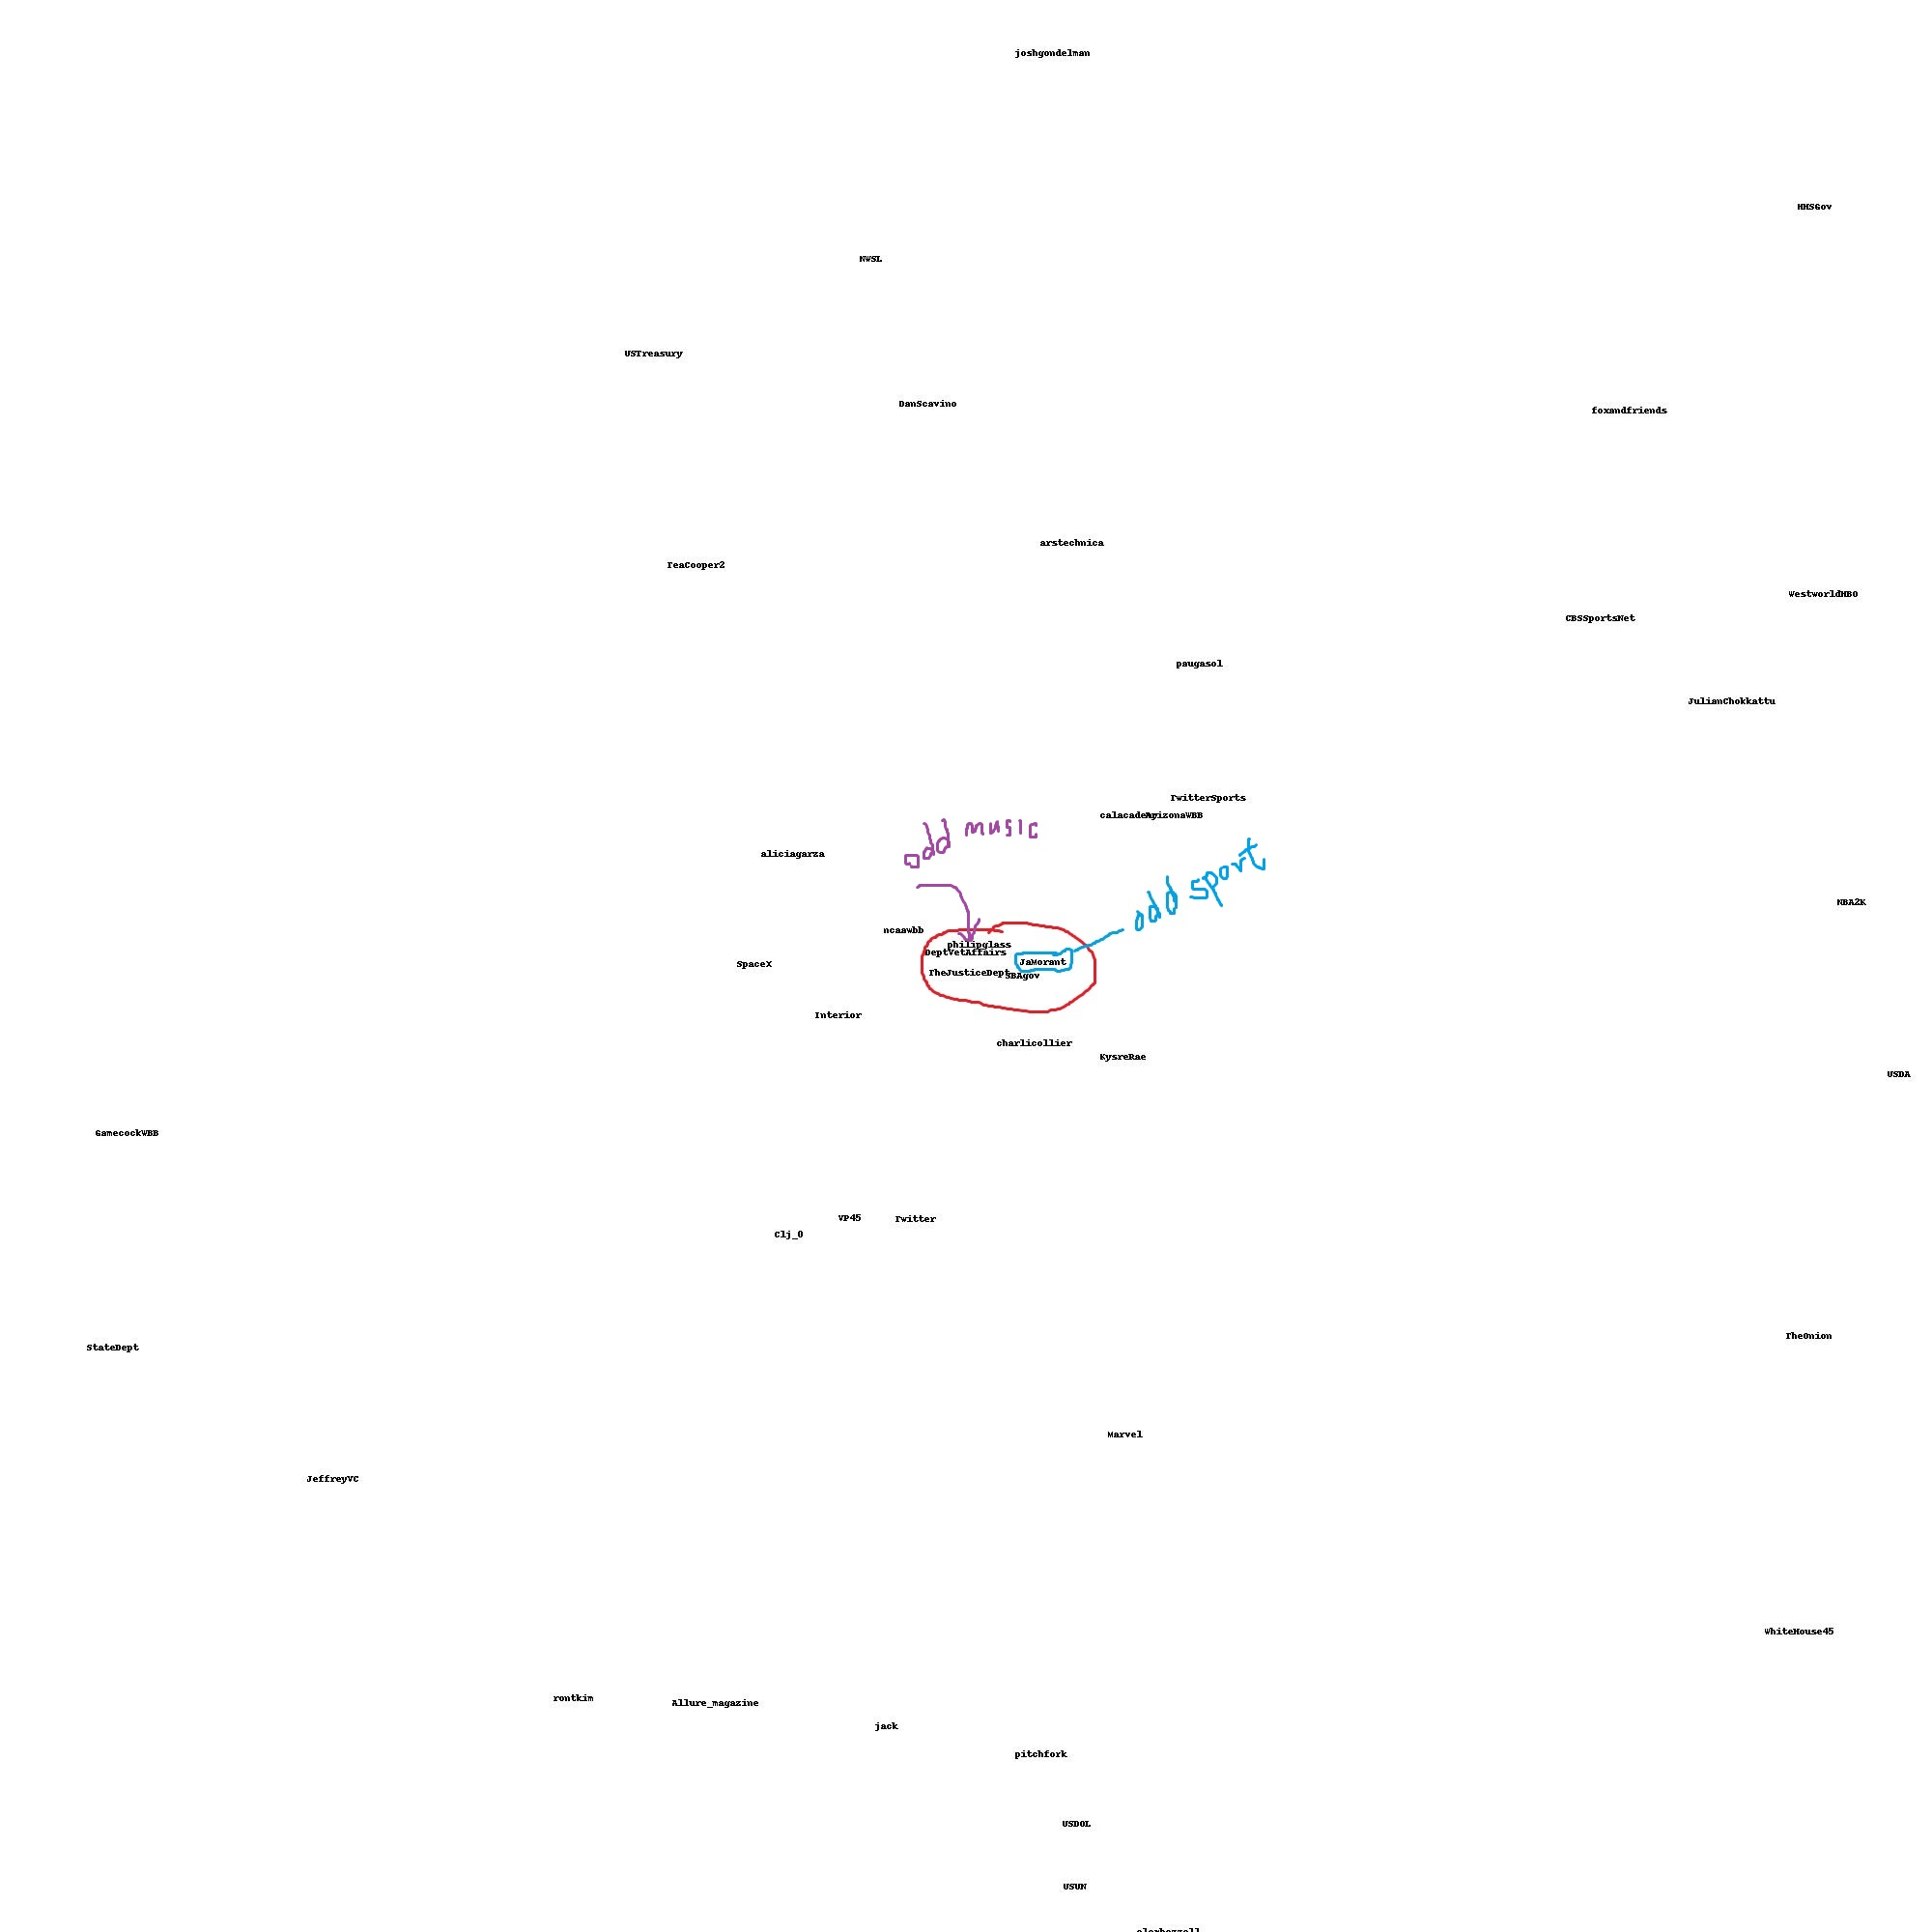
\includegraphics[width=\textwidth,height=\textheight,keepaspectratio]{tweets2d.jpg}
            \caption{ MDS Image Question 5}
            \label{fig:3}
\end{figure}
\subsection*{Discussion}
\emph{I had the following result:}
    \begin{itemize}
        \item There were 98 iteration in total by checking the length of coord in line 486
         \lstinputlisting[language=Python,caption= A snapshot question3.py cluster 20 showing iterations and cluster summary, label=Q5alist:import,firstnumber=477,firstline=477,lastline=487]{question3.py}
        \item MDS did fairly good but there was a group containing two particular odd group members \href{https://twitter.com/JaMorant?s=20}{Jamorant} (Sport category) and 
    \href{https://twitter.com/philipglass?s=20}{philipglass}(Music category), the two were odd because the group was filled with mostly political screen names.
        \item For the code to work, we would have to read in the tweetdata.txt and parse in the data variable into scaledown(data) function. The functions are from the lecture notes. The function
scaledown  then creates the file tweets2d.jpg Figure \ref{fig:3}.
        \item I remember running into and error when I parse in data in the scaledown() function.
        \begin{lstlisting}
        errorterm = (fakedist[j][k] - realdist[j][k]) / realdist[j][k]
        ZeroDivisionError: float division by zero
        \end{lstlisting}
        Apparently when the code was calculating teh percentage difference between the distance of two pairs, result in a zero value which should not be the case.
        This meant that one of my screen\_names() the \href{https://twitter.com/Cabinet45}{Cabinet45} in account-term matric had an output of all zeros values. (View \href{https://github.com/cs432-websci-spr21/hw8-cluster-aaden001/blob/master/tweetdataWithCabinet45.txt}{tweetdataWithCabinet45.txt in github line 80} )
    \end{itemize}
\section*{References}
\begin{itemize}
    \item {\url{https://stackoverflow.com/questions/48230230/typeerror-mismatch-between-array-dtype-object-and-format-specifier-18e/48231106}}
     \item {\url{https://www.kite.com/python/answers/how-to-write-contents-of-a-dataframe-into-a-text-file-in-python}}
     \item{\url{https://www.geeksforgeeks.org/remove-last-n-rows-of-a-pandas-dataframe/}}
     \item{\url{https://www.geeksforgeeks.org/python-pandas-dataframe-drop_duplicates/}}
     \item{\url{https://www.geeksforgeeks.org/how-to-add-one-row-in-an-existing-pandas-dataframe/}}
     \item{\url{https://stackoverflow.com/questions/10897339/python-fetch-first-10-results-from-a-list}}
     \item{\url{https://stackoverflow.com/questions/22412258/get-the-first-element-of-each-tuple-in-a-list-in-python}}
\end{itemize}

\end{document}

